\section{Introduction}
\label{sec:introduction}

%%%
%%% intuition // generative vs discriminative
%%%
Intuitively, generative modeling is based on the idea that in order to produce data similar to samples from a dataset it helps to understand the data first~\cite[p.~720]{deeplearning:2016}.
%The case of deep learning suggests the use of deep, hierarchical architectures to capture dependencies within the data and reduce the high-dimensional input~\cite{reducing_dim:2006}.
In contrast to discriminative models which model the conditional distribution $p(y|x)$ of the labels $y$ given observations $x$, generative algorithms model the joint distribution $p(x,y)$ over both labels and observations to describe how the data was generated~\cite{learning_dbn:2006}.
As there are only observations given, the generative task seems more difficult than classification where both input and desired output are given during training.~\cite[p.~695]{deeplearning:2016}\\\\
%
Due to the nature of generative models, they are unsupervised learning algorithms which mean that they try to learn the structure of samples from an unlabeled dataset\cite[p.~105-106]{deeplearning:2016}\cite{prob_unsupervised:1999}.
%
Generative models in machine learning using probabilistic models can be mostly separated into directed and undirected models~\cite[p.~77]{deeplearning:2016}.
%
This separation indicates how the model can be mapped to a graph with random variables as vertices and interactions between random variables as edges.
Directed models induce a directed network graph while undirected models induce a network graph with undirected edges.\\\\
%
%
In directed models, we assume that the observations $x$ are stochastically dependent on the underlying factors, also called latent variables $z$. This relationship can be expressed as the graphical model shown in Figure~\ref{fig:dgm}.
Note that the latent variables can be structured hierarchically in order to express different levels of granularity in the features of the underlying factors and representations~\cite[p.~557]{deeplearning:2016}.
\begin{figure}[htb]
\centering
  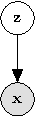
\includegraphics[width=1.3cm]{media/directed_graphical_model}
  \caption[Graphical Model]{Directed Graphical Model}
\label{fig:dgm}
  \medskip
  \small
  The observed data $x$ is stochastically dependent on the latent variables $z$.\\
  Based on~\cite[Chapter 8]{bishop:2006}.
\end{figure}



\subsection{Overview}
% traditional models (HMM, GMM)
Traditional models include hidden Markov models used for example in speech recognition~\cite{hmm:1989}, which are generative models~\cite[p.~878]{modern_approach:2009} and Gaussian mixture models~\cite[p.~190]{deeplearning:2016}\cite{schuster:1999}.\\\\
%
% undirected networks (Boltzmann machine)
Undirected generative models include various extensions of the Boltzmann machine~\cite{bm:1985} such as the restricted Boltzmann machine (RBM), first described as Harmonium~\cite{smolensky:1986} and the deep Boltzmann machine~\cite{dbm:2009}\cite[Chapter~20.4]{deeplearning:2016}.\\\\
%
% directed networks (SBN, DBN)
For directed models, the sigmoid belief network (SBN) is an early model described in 1992~\cite{neal:1992} which is presented in Section~\ref{sec:sbn}.
SBN has also been extended with a restricted Boltzmann machine for the first two layers resulting in deep belief nets (DBN)~\cite{learning_dbn:2006}, which have been attributed to spark the beginning of current deep learning~\cite[p.~662]{deeplearning:2016}. DBN are partially directed models, as they contain both directed and undirected connections~\cite[p.~664]{deeplearning:2016}.\\\\
%
%Another class of generative models are auto-regressive networks (ARN), which 
%\newpage
%%%
%%% applications
%%%

\subsection{Applications}


\begin{figure}[t]
  \includegraphics[width=\linewidth]{media/caption2img}
  \caption[Caption-to-Image Samples]{Generative Text to Image Synthesis~\cite{gan_t2i:2016}}
  \medskip
  \small
  The top row shows the provided captions and in the bottom row the corresponding synthesized images.
\label{fig:caption2img}
\end{figure}


Generative models learn the joint distribution $p(x,y)$ and due to this fact they can be used to perform classification as well by expand $p(x,y)$ to $p(y|x)$ as indicated by Equation~\ref{eq:class}.
\begin{equation}
  \label{eq:class}
  p(y|x) = \frac{p(x,y)}{p(x)}
\end{equation}
%
One obvious application of generative models is to use the model to sample more data similar to samples from a given training dataset.\\
%
In computer vision tasks, generative models have been largely outperformed by much simpler models until at least 2011~\cite{thesis:2011}. In 2015 however, convolutional networks have been shown to surpass those models in image synthesis~\cite{synthesis:2015}.
Other tasks involving image modeling include performing super-resolution~\cite{superres:2017}, constructing 3D models from 2D images~\cite{gan_3d:2016}, predicting the next video frames~\cite{gan_video:2016}, and synthesizing new images from captions as shown in Figure~\ref{fig:caption2img}.\\
%
In the area of reinforcement learning, generative models offer a way to perform action space exploration~\cite{rl_variational:2016}. Generative adversarial networks discussed in Section~\ref{sec:gan} have been shown to be used in imitation learning, where the generative model is used to imitate previously seen interactions~\cite{imitation_learning:2016}.\\
%
SampleRNN~\cite{samplernn:2016}, which is a recurrent neural network combined with an auto-regressive network have been shown to produce good generated audio samples.\\\\
%
Recently, generative models have also shown to improve semi-supervised learning performance significantly~\cite{cvae:2014}. Semi-supervised learning algorithms use only small amount of labeled data, which is usually difficult to obtain and large amounts of unlabeled data, which is easier to obtain in most cases.



\newpage
